%______________________________________________________________________________
% main.tex

\input{preamble12-screen.tex}
\hypersetup{%
    pdfauthor={Mike Pierce}%
   ,pdftitle={Math N16B Eight Eight, Summer 2021}%
   ,pdfkeywords={Pierce,MathN16B,16B,N16B,Calculus,Integration,Berkeley}%
}
\usepackage{fourier}
\input{accessible-colors.tex}
\input{newcommand.tex}
\input{newenvironment.tex}
\pagestyle{empty}


\begin{document}

\begin{center}
    {\Huge{Homework Eight}}
    \\ \footnotesize{Analytic Geometry and Calculus}
    \\ \footnotesize{UC Berkeley Math N16B, Summer 2021}
\end{center}
\vspace{2em}

These exercises you should complete at your discretion.
Note that \emph{Calculus with Applications, 11th Edition} 
has some select solutions, usually to odd-numbered exercises, in the back.


\section*{Goals this Week}

Here are some goals you should have in mind while exercising:
\begin{enumerate}
    \item 
        Know what a geometric series is, either finite or infinite, 
        and know the formula for its value.

    \item 
        \textsc{Know what a Taylor series is}!
        Appreciate their importance.
        This is literally one the most useful things ever:
        you can manually approximate transcendental numbers like $\ex$ with these!
        (You should know how to do this, like in the last exercise 
        on this homework)
        You should know the general formula for a Taylor series,
        and also commit to temporary memory the Taylor series for
        the functions $\ex^x$ and $\inv{(1-x)}$ and $\ln(1+x)$
        and their intervals of convergence.
        Develop some comfort doing arithmetic on Taylor series
        and composing Taylor series; 

    \item 
        \emph{Newton's method} is a great way to estimate roots (zeros)
        of a function. It's an algorithmic method though,
        and should really only be implemented using a computer,
        so there's no need to do any exercises over it.
        But you should certainly understand the idea behind Newton's method.

\end{enumerate}

\newpage

\section*{Exercises}

\begin{enumerate}
    \item % 12.1 Sequences and Series and 12.4 Infinite Series
        The initial exercises from Chapter 12.1 \& Chapter 12.4
        \emph{Calculus with Applications, 11th Edition}
        will help you internalize what a geometric series is,
        and how to calculate the explicit value of such a series,
        whether it's finite or infinite.
        Do them.

    \item Some ``application'' questions from the textbook.
        \begin{center}
            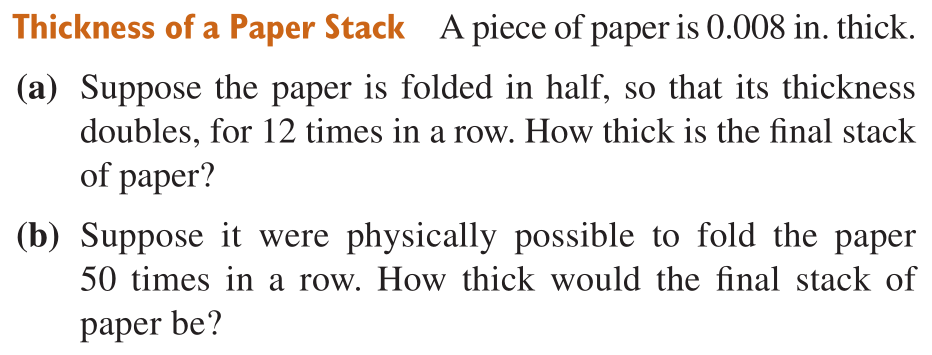
\includegraphics[width=0.96\textwidth]{screenshots/thicc.png}
            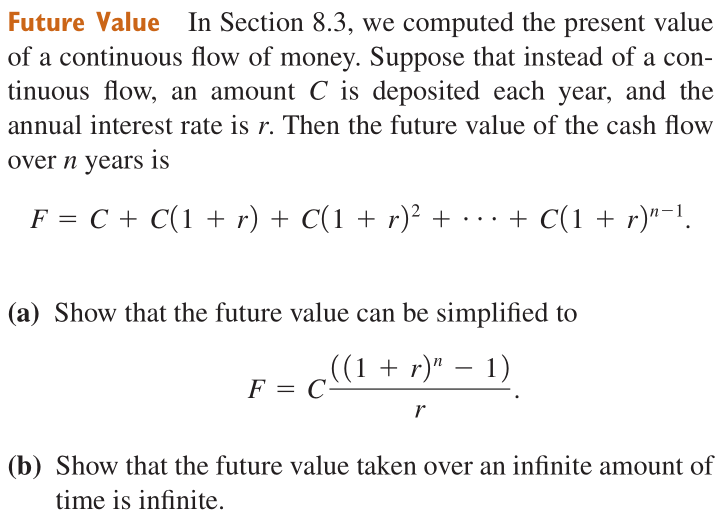
\includegraphics[width=0.96\textwidth]{screenshots/value.png}
            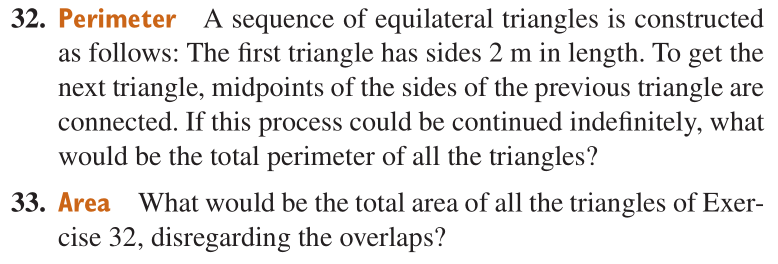
\includegraphics[width=0.96\textwidth]{screenshots/triangles.png}
            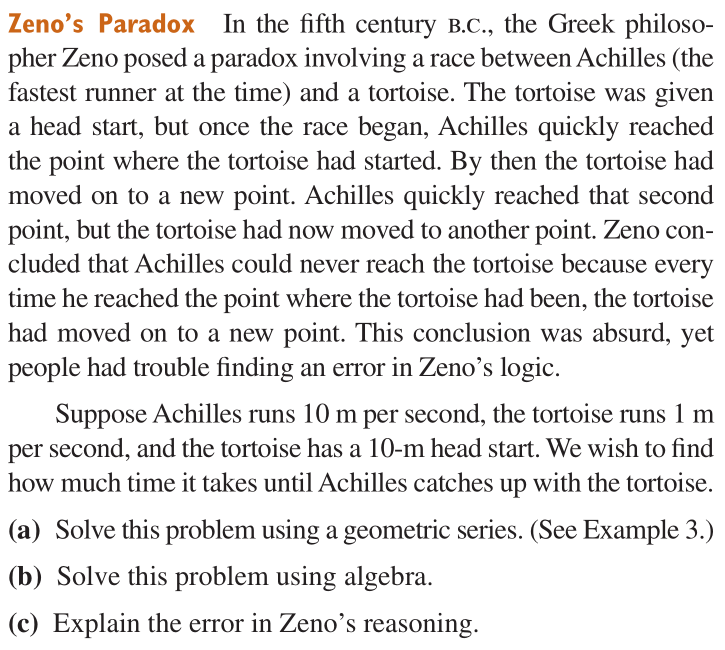
\includegraphics[width=0.96\textwidth]{screenshots/zeno.png}
        \end{center}

    \item % 12.5 Taylor Series
        I expect you to know the Taylor series for
        the functions $\ex^x$ and $\inv{(1-x)}$ and $\ln(1+x)$
        and feel comfortable doing some arithmetic with them.
        The initial exercises from Chapter 12.5 of 
        \emph{Calculus with Applications, 11th Edition}
        provides you with some practice with this.

    \item 
        Compute the Taylor series centered at $0$ for the functions
        sine and cosine. The radius of convergence for each of these
        series is $(-\infty, \infty)$.
        Up until this point you've had to trust that the derivative 
        of sine is cosine, and that the derivative of cosine 
        is negative sine, but now you have the tools to prove this!
        Using just the power rule, verify that 
        \begin{equation*}
            \ddx \cos(x) = -\sin(x)
            \quad\text{and}\quad
            \ddx \sin(x) = \cos(x)
            \,.
        \end{equation*}
        Once you've done this, using their Taylor series, verify that
        \begin{equation*}
            \cos(x) = \frac{\ex^{\im x} + \ex^{-\im x}}{2}
            \quad\text{and}\quad
            \sin(x) = \frac{\ex^{\im x} - \ex^{-\im x}}{2i}
        \end{equation*}
        where $\im^2 = -1$.

    \item 
        Using the appropriate Taylor series,
        demonstrate how you can, using only pencil and paper, 
        find rational approximation to any of the following numbers 
        with as much precision as you desire.
        \begin{equation*}
            \sin(3) \qquad\qquad \ln(2) \qquad\qquad \ex
        \end{equation*}

\end{enumerate}

\end{document}

